\documentclass[12pt]{report}
\raggedright
\parindent0pt \parskip8pt
\usepackage{graphicx}

\begin{document}

\begin{Huge}
\begin{center}
\begin{normalsize}
\textbf{MAKERERE 
\includegraphics[scale=0.5]{logo} UNIVERSITY }\\


\textbf{FACULTY OF COMPUTING AND INFORMATICS TECHNOLOGY} \\
\textbf{SCHOOL OF COMPUTING AND INFORMATICS TECHNOLOGY} \\
\textbf{DEPARTMENT OF COMPUTER SCIENCE} \\
\textbf{BACHELOR OF SCIENCE IN COMPUTER SCIENCE} \\
\textbf{YEAR 2} \\
\textbf{BIT 2207 RESEARCH METHODOLOGY} \\
\textbf{Course Work: Assignment 5}\\
\end{normalsize}
\end{center}
\end{Huge}

\begin{center}
\begin{tabular}{|l|l|l|c|}
\hline NAME  & REG NO & STD NO \\\hline
OKOT EMMANUEL& 16/U/10916/PS & 216015844 \\\hline
MASIGA DAVID KELVIN& 16/U/579 & 216000507 \\\hline
NABWIRE BABRA SANDRA& 16/U/10916/PS & 216011336 \\\hline
MULINDWA MATOVU KENNEDY& 16/U/10916/PS & 216021701 \\\hline
\end{tabular}
\paragraph{•}
GROUP F\\
\paragraph{•}
Lecturer: ERNEST MWEBAZE \\
\paragraph{•}
8th March 2018

\end{center}

\newpage

\title{SPEEDING DETECTOR ALONG ROADS TO CURB INCREASING ROAD TRAFFIC ACCIDENTS IN UGANDA IN VIEW OF TAXI DRIVERS}
\author{By Group F}      
\renewcommand{\today}{}

\maketitle
\tableofcontents

\chapter{Introduction}
\section{Background}
\paragraph{•}
Barely two months after 13 Tanzanian nationals perished on the Kampala-Masaka highway after attending a wedding in Kamoala, one Ugandan has died and three others were badly injured in an accident, on same road. Eye witnesses said the speeding FUSO truck lost control in a "dangerous spot" and swayed towards the side of the oncoming Saloon car, causing the crash at about 10:00pm. The car was damaged beyond repair. The driver of the Sallon car was travelling together with three passengers when this occurred. The three sustained serious injuries while the driver died on the scene.\cite{newvision} 
\paragraph{•}
Though the cause of the accident is still being investigated, road accidents have claimed the lives of many individuals, and is among the leading causes of injuries that are treated in a very odd way. Low income countries (LIC) and middle income countries (MIC) populations are faced with more road deaths than the high income countries (HIC) but all are as much affected.
\paragraph{•}
Regardless of what level of income an individual is, all road users are at risk of this endemic. The most hurting accidents are those that claim the life of children or pedestrians who are caught in the indiscipline of drivers to keep or maintain traffic rules. 
\paragraph{•}
Research has it that there are very many causes for road accidents; including - driver's age, weather, road conditions, driver's sex, drunkenness, attitudes of drivers and so on.\cite{hellen} Traffic experts agree that a good driving attitude-more than driving skill-can keep you out of most accident-producing situations from which not even the most skillful driver could escape without injury or property loss.\cite{stone} By observation, taxi drivers are well known for exhibiting a very bad attitude while driving. All these causes of accidents can be categorized as human error, environment factors and vehicle factors. In Uganda the process of tracking and  monitoring the behavior of drivers  has always been done  by the  traffic  officers  who often stand alongside roads and highways in specific areas using speed guns and radar antennas to catch over 
speeding  vehicles.  This  was  put  in  practice  after  sighting  over  speeding  as  one  of  the  main  causes  of  road accidents  by  the  traffic  police  of  Uganda  (Mubaraka,  2013).  However,  these  traffic  officers  cannot  be assembled in all spots of the roads to control the traffic. This has left the lives of very many Ugandans using road transport especially public transport at the mercy of irresponsible drivers.\cite{mukreport} The purpose of this research is to help improve the safety of passengers by designing a system that can be installed along blind spots to capture information on over speeding vehicles and report to the traffic police automatically.

\section{Lessons from Domestic and International Speed Camera Programs}
\paragraph{•}
Most researchers and public safety officials agree that speeding causes an increase in crashes. They generally agree that speed limit enforcement measures, including cameras, help catch and penalize drivers who break that speed limit. However, some questions remain unanswered. Do speed cameras actually lead to a reduction in the number of speeders and crashes, or reduce crash severity overall? \cite{boos}
\paragraph{•}
It has been an observation of many that when drivers are well acquainted with roads and visible speed cameras, as they approach an enforcement zone, they suddenly decelerate only to accelerate again after having passed it. There is no experimental proof that this leads to accidents however drivers will not have learned the detrimental results over speeding could lead to. In addition, some research has noted that drivers aware of fixed speed cameras may resort to using alternative routes to avoid the cameras, possibly leading to an increase in crashes on other roadways.
\paragraph{•}
Many drivers have actually discovered that not all speed cameras work, some are switched off. For this reason, speed cameras are actually ignored by such drivers.

\section{Problem Statement}
\paragraph{•}
Currently the Uganda traffic police use radar speed guns to detect over speeding vehicles. Traffic officers are deployed alongside roads, highways or streets to detect and stop over speeding vehicles. However, drivers exploit the loopholes within the current operational systems by reducing speed in areas where they suspect officers to be. This therefore does not reduce the over speeding and accident problems. The current traffic tracking system in Uganda has weaknesses which include the following;
\begin{itemize}
\item There are limited numbers of traffic officers therefore not enough to deploy on all roads in the entire country.
\item The cost of speed guns is high therefore this makes it hard to purchase them for every traffic officer. Consequently, just a few traffic officers possess speed guns. \cite{mukreport}
\end{itemize}
\paragraph{•}
While successful speed detector programs are in place in many countries today, the use of enforcement speed detectors is certainly contentious. Many international programs were initially met with public resistance. There are a number of public concerns transportation professionals may want to contemplate when considering or implementing a speed detector, including: general ticketing procedures, how ticket revenues will be distributed, privacy issues, and whether or not automated enforcement does result in reduced crash rates. Some studies have noted that public resistance to such programs can occur if speed detectors are perceived as revenue generators rather than methods for improving safety.
\paragraph{•}
In solving the problem of traffic violations along blind spots on different highways, the installation of speed detectors will be carried out in areas where traffic officers will be deployed and where they are not. On the upper hand, limitations in the number of traffic officers will be reduced. However, the cost to be incurred in the purchase of these devices will rise. 

\section{Objectives}
\subsection{General Objectives}
\paragraph{•}
The speed detectors should be able to function both in the day and in the night. The module must be able to capture the image of a vehicle violating traffic rules, process the it's plate number and match the vehicle with a list of other vehicles to process what mode of vehicle it is. The geographical scope includes all major highways such as Kampala-Mbarara, Kampala-Mbale, Kampala-Entebbe highways e.t.c. in Uganda. In the long run, the system will improve the measures of effectiveness of road safety education, training and publicity projects.
\subsection{Specific Objectives}
\paragraph{•}
To critically analyze the current traffic tracking process in order to identify requirements for the system. Every speed detector should be configured manually by the traffic law enforcers, to identify the requirements for each blind spot along the road.
\paragraph{•}
To design, implement, test and validate the vehicle speed tracking and reporting system. The system should be able to track speeding vehicles and generate reports for the traffic police.
The system is not meant for for other means of public transport such as air, railway or water transport.
\paragraph{•}
The system will help traffic police identify and penalize over speeding vehicles thus reducing accidents. The research will also provide source of revenue to the government through the fines charged on over speeding drivers. The money collected from fines for over speeding will go to the Uganda Revenue Authority for other development projects by the government including the maintenance of this project.
\section{Methodology}
\paragraph{•}
Data was collected through the use of interviews, literature review and observation. Interviews were conducted with students. Observation method helped make informed decisions, adjustments and allowances based on what had been studied. The researchers saw how traffic officers track over speeding vehicles along high ways. Analysis of this collected data was done using Microsoft Excel because it features calculation, graphing tools among others. A Data Flow Diagram (DFD) was used for system design.
\subsection{System Analysis}
\paragraph{•}
MS Excel was used to analyze data and results show 25\% needed more education about the system and 75\% of the respondents were willing to install the speed detectors along the road. 70\% of respondents rated the system excellent, 20\% rated it to be very excellent while 10\% had no idea about the system.
\begin{figure}[ht]
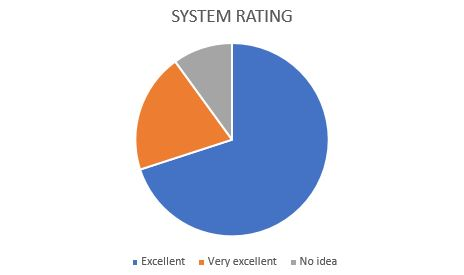
\includegraphics[]{Piechart}
\caption{How the System was rated}
\end{figure}
\paragraph{•}
According to literature review, 50\% of road accidents are due to over speeding of public vehicles on highways and other factors also contribute 50\% of total accidents recorded per year.\cite{mukreport}
\subsection{System Design}
\paragraph{•}
The functional requirements identified include traffic officers entering in the speed limit of the highway. On automatic system input of driver's registration number, tracking speed in real time, and a notification to the traffic head office is automatically sent, identifying errors. The system generates an alert to any available user incase the speed goes beyond the recommended speed limit set.
\paragraph{•}
The non functional requirements include a system with quick response and the system should temporarily store the session and resume without interference.
\section{System Architecture}
\paragraph{•}
Process modeling is a formal way of presenting how the system operates. The context diagram shows how data moves through the information system.
\begin{figure}[ht]
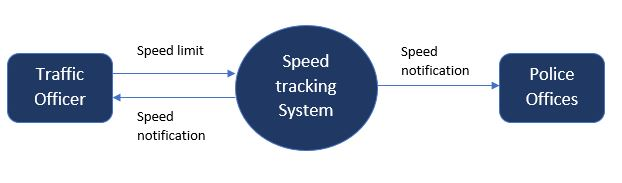
\includegraphics[scale=0.8]{dfd}
\caption{Context diagram showing system overview}
\end{figure} 
\section{Results}
\paragraph{•}
The functionalities of the system include detecting approaching vehicles, tracking speed in real time and automatically sending notifications of the driver's vehicle model and plate number in case of over-speeding, fast in speed and temporarily stores the session in case of disruption and resumes when the problem addressed.
\begin{itemize}
\item The speed detector uses character recognition and captures the number plate from the scan, stores the picture to process its car type.
\item The speed detector is labeled with a unique number and generally monitored at the police offices where the unique number is matched to its location, hence no need for GPS tracking.
\end{itemize}
\section{Conclusion}
\paragraph{•}
The problem of road accidents will reduce to some extent thereby saving a big percentage of lives lost every day in Uganda.
\begin{thebibliography}{9}
\bibitem{newvision} Eddie Ssejjoba. "One dead, three injured on Kampala-Masaka highway" www.newvision.co.ug/new\_vision/news/1465158/dead-injured-kampala-masaka-highway, Nov. 6, 2017 [March 14, 2018]
\bibitem{hellen} Hellen Nnajjuma. "Road Traffic Accidents in Uganda in view of Taxi Drivers Masaka District." M.A thesis, Trondheim, Autumn 2013.
\bibitem{stone} Alfred R. Stone. \textit{Caution: Driving Ahead}, Texas, 
Steck-Vaughn,1974,pp. 28.
\bibitem{boos} Misty A. Boos. "Speed Cameras as a Tool to Reduce Road Fatalities" \textit{Research Synthesis Bibliographies}, vol. 23, 2009
\bibitem{mukreport} Kamoga Meddy4, Emily Bagarukayo, Kanani Ronald, Natugasha Dennis, Arinda Yvonne. "\textit{Vehicle Speed Tracking and Reporting System for Uganda}", Makerere University, Uganda, 2015.

\end{thebibliography}
\end{document}